\documentclass[12pt,a4paper]{article}

% Packages
\usepackage{geometry}
\geometry{margin=1in}
\usepackage{fancyhdr}
\usepackage{titlesec}
\usepackage{listings}
\usepackage{xcolor}
\usepackage{graphicx} 

% Header & Footer
\pagestyle{fancy}
\fancyhf{}
\rhead{C++ - Assignment 3}
\lhead{Kamithkar Vinod}
\cfoot{\thepage}

% Title formatting
\titleformat{\section}{\large\bfseries}{Problem \thesection:}{0.5em}{}
\titleformat{\subsection}[runin]{\bfseries}{Code:}{0.5em}{}[---]
\titleformat{\subsubsection}[runin]{\bfseries}{Output:}{0.5em}{}[---]

% Code style
\lstset{
    language=cpp,
    basicstyle=\ttfamily\small,
    keywordstyle=\color{blue}\bfseries,
    commentstyle=\color{gray}\itshape,
    stringstyle=\color{red},
    showstringspaces=false,
    numbers=left,
    numberstyle=\tiny\color{gray},
    frame=single,
    breaklines=true
}

% Document Start
\begin{document}

% Title Page
\begin{center}
    \LARGE \textbf{Assignment - 3} \\[0.5cm]
    \Large \textbf{C++} \\[1cm]

    \begin{tabular}{rl}
        \textbf{Name:} & Kamithkar Vinod \\
        \textbf{Course:} & PG DAC AUGUST 2025 \\
        \textbf{PRN:} & 250850320040 \\
        \textbf{Form No:} & 250500480 \\
        \textbf{Date:} & 09-10-2025 \\
    \end{tabular}
\end{center}

\vspace{1cm}
\hrule
\vspace{0.5cm}

% Problems
% 1
\section{Basic Class}
\textbf{Task:} Write a program in C++ to create a class Car with data members name and speed.
    \item - Use a member function display() to print values.
    \item - Create two objects and display their details.


\subsection{}
\begin{lstlisting}
#include <iostream>
using namespace std;

class Car {
    string name;
    int speed;

public:
    void setData(string n, int s) {
        name = n;
        speed = s;
    }

    void display() {
        cout << "Car Name: " << name << endl;
        cout << "Speed: " << speed << " km/h" << endl;
    }
};

int main() {
    Car c1, c2;
    c1.setData("BMW", 220);
    c2.setData("Audi", 200);

    cout << "Car 1 Details:" << endl;
    c1.display();
    cout << "\nCar 2 Details:" << endl;
    c2.display();
    return 0;
}


\end{lstlisting}

\subsubsection{1}
\begin{center}
    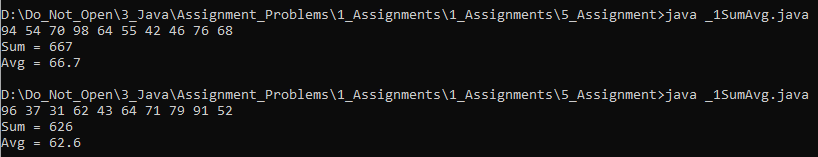
\includegraphics[width=0.8\textwidth]{1.png}
\end{center}


% 2

\section{Rectangle (Area & Perimeter)}
\textbf{Task:} Create a class Rectangle with data members length and width.
    \item ● Add member functions to calculate area and perimeter.
    \item ● Read values from user and display results.
\subsection{}
\begin{lstlisting}
#include <iostream>
using namespace std;

class Rectangle {
    float length, width;

public:
    void input() {
        cout << "Enter length and width: ";
        cin >> length >> width;
    }

    float area() {
        return length * width;
    }

    float perimeter() {
        return 2 * (length + width);
    }

    void display() {
        cout << "Area: " << area() << endl;
        cout << "Perimeter: " << perimeter() << endl;
    }
};

int main() {
    Rectangle r;
    r.input();
    r.display();
    return 0;
}


\end{lstlisting}

\subsubsection{}
\begin{center}
    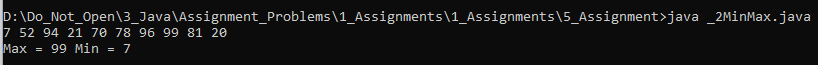
\includegraphics[width=0.8\textwidth]{2.png}
\end{center}

% 3

\section{Student Details}
\textbf{Task:} Create a class Student with data members rollNo, name, and marks.
    \item ● Add member function input() to take values.
    \item ● Add function display() to print them.
    \item ● Create an array of 3 students and display all details. 

\subsection{}
\begin{lstlisting}
#include <iostream>
using namespace std;

class Student {
    int rollNo;
    string name;
    float marks;

public:
    void input() {
        cout << "Enter Roll No, Name, and Marks: ";
        cin >> rollNo >> name >> marks;
    }

    void display() {
        cout << "Roll No: " << rollNo << ", Name: " << name << ", Marks: " << marks << endl;
    }
};

int main() {
    Student s[3];
    cout << "Enter details for 3 students:\n";
    for (int i = 0; i < 3; i++) {
        s[i].input();
    }

    cout << "\nStudent Details:\n";
    for (int i = 0; i < 3; i++) {
        s[i].display();
    }
    return 0;
}

\end{lstlisting}

\subsubsection{}
\begin{center}
    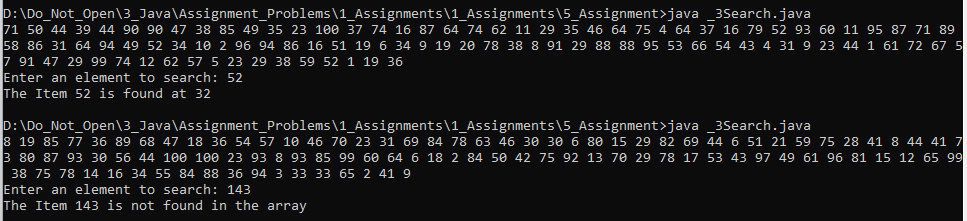
\includegraphics[width=0.8\textwidth]{3.png}
\end{center}

% 4

\section{Bank Account}
\textbf{Task:} Create a class BankAccount with:
    \item ● Data members: accountNumber, balance.
    \item ● Functions: deposit(), withdraw(), displayBalance().
    \item ● Perform deposit and withdrawal operations using objects.

\subsection{}
\begin{lstlisting}
#include <iostream>
using namespace std;

class BankAccount {
    int accountNumber;
    double balance;

public:
    void openAccount(int accNo, double bal) {
        accountNumber = accNo;
        balance = bal;
    }

    void deposit(double amount) {
        balance += amount;
        cout << "Deposited: " << amount << endl;
    }

    void withdraw(double amount) {
        if (amount <= balance) {
            balance -= amount;
            cout << "Withdrawn: " << amount << endl;
        } else {
            cout << "Insufficient balance!" << endl;
        }
    }

    void displayBalance() {
        cout << "Account Number: " << accountNumber << ", Balance: " << balance << endl;
    }
};

int main() {
    BankAccount acc1;
    acc1.openAccount(1001, 5000);
    acc1.deposit(2000);
    acc1.withdraw(1500);
    acc1.displayBalance();
    return 0;
}
\end{lstlisting}

\subsubsection{}
\begin{center}
    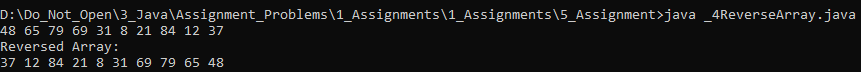
\includegraphics[width=0.8\textwidth]{4.png}
\end{center}

% 5

\section{Employee Salary (Parameterized Constructor) }
\textbf{Task:} Write a C++ program to create a class Employee with data members id, name, and salary.
    \item ● Use a parameterized constructor to initialize values.
    \item ● Display employee details using a function.

\subsection{}
\begin{lstlisting}
#include <iostream>
using namespace std;

class Employee {
    int id;
    string name;
    float salary;

public:
    Employee(int i, string n, float s) {
        id = i;
        name = n;
        salary = s;
    }

    void display() {
        cout << "ID: " << id << ", Name: " << name << ", Salary: " << salary << endl;
    }
};

int main() {
    Employee e1(101, "Vinod", 50000);
    Employee e2(102, "Kumar", 60000);

    e1.display();
    e2.display();
    return 0;
}


\end{lstlisting}

\subsubsection{}
\begin{center}
    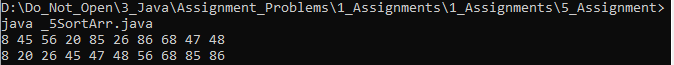
\includegraphics[width=0.8\textwidth]{5.png}
\end{center}

% 6

\section{Complex Number (Object as Argument) }
\textbf{Task:} 
Create a class Complex with data members real and imag.
    \item ● Add a member function add() that takes another Complex object and returns the result as a new
object.
    \item ● Display the sum of two complex numbers.

\subsection{}
\begin{lstlisting}
#include <iostream>
using namespace std;

class Complex {
    float real, imag;

public:
    void input() {
        cout << "Enter real and imaginary parts: ";
        cin >> real >> imag;
    }

    Complex add(Complex c2) {
        Complex temp;
        temp.real = real + c2.real;
        temp.imag = imag + c2.imag;
        return temp;
    }

    void display() {
        cout << real << " + " << imag << "i" << endl;
    }
};

int main() {
    Complex c1, c2, c3;
    cout << "Enter first complex number:\n";
    c1.input();
    cout << "Enter second complex number:\n";
    c2.input();

    c3 = c1.add(c2);

    cout << "Sum of complex numbers: ";
    c3.display();
    return 0;
}


\end{lstlisting}

\subsubsection{}
\begin{center}
    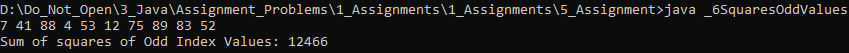
\includegraphics[width=0.8\textwidth]{6.png}
\end{center}

% 7

\section{Library Management}
\textbf{Task:} 
Create a class Book with data members title, author, and price.
    \item ● Write functions to input and display details.
    \item ● Create an array of 5 books and print the book with the highest price.

\subsection{}
\begin{lstlisting}
#include <iostream>
using namespace std;

class Book {
    string title, author;
    float price;

public:
    void input() {
        cout << "Enter Title, Author, and Price: ";
        cin >> title >> author >> price;
    }

    void display() {
        cout << "Title: " << title << ", Author: " << author << ", Price: " << price << endl;
    }

    float getPrice() {
        return price;
    }
};

int main() {
    Book b[5];
    cout << "Enter details for 5 books:\n";
    for (int i = 0; i < 5; i++) {
        b[i].input();
    }

    int maxIndex = 0;
    for (int i = 1; i < 5; i++) {
        if (b[i].getPrice() > b[maxIndex].getPrice())
            maxIndex = i;
    }

    cout << "\nBook with Highest Price:\n";
    b[maxIndex].display();
    return 0;
}


\end{lstlisting}

\subsubsection{}
\begin{center}
    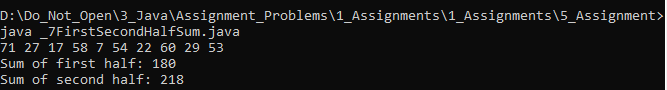
\includegraphics[width=0.8\textwidth]{7.png}
\end{center}



\end{document}



